\documentclass[12pt, twoside, openany]{report}
\usepackage{graphicx}
\usepackage{a4wide}
\usepackage[utf8]{inputenc}
\usepackage{enumerate}
\usepackage{verbatim}
\usepackage[polish,british]{babel}
\usepackage[T1]{fontenc}
\usepackage{geometry}
\geometry{left=25mm,right=25mm,%
bindingoffset=10mm, top=25mm, bottom=25mm}
\usepackage{latexsym}
\usepackage{amsthm}
\usepackage{palatino}
\usepackage{array}
\usepackage{csquotes}
\usepackage{textcomp}
\theoremstyle{definition}

\setcounter{tocdepth}{1}
\newcommand*{\norm}[1]{\left\Vert{#1}\right\Vert}
\newcommand*{\abs}[1]{\left\vert{#1}\right\vert}
\newcommand*{\om}{\omega}

\author{Paweł Paczuski}
\title{Tytuł pracy}

\begin{document}

% Zażółć gęślą jaźń.
\begin{titlepage}
\pagestyle{empty}

\noindent
\begin{Large}
\begin{table}[t]
\centering
\begin{tabular}[t]{lcr}
 
\includegraphics[width=70pt,height=70pt]{pw} & Warsaw University of Technology & 
\includegraphics[width=70pt,height=70pt]{elka}\\
& FACULTY OF & \\
& ELECTRONICS AND INFORMATION TECHNOLOGY &
\end{tabular}
\end{table}

% \vfill
\begin{center}BACHELOR'S DIPLOMA THESIS\end{center}
\begin{center}In the field of Computer Science \\ and specialization Computer Systems and Networks \end{center}\end{Large}
% \vfill
\begin{center}
\Huge
\textbf{!!!DRAFT!!! Structured reporting system}
\end{center}
% \vfill\vfill
\vfill
\begin{center}
\Large
Author:\\
\LARGE
Paweł Paczuski
\end{center}
\vfill
\begin{center}
\Large
Thesis supervisor: Jan J. Mulawka PhD, DSc
\end{center}
\vfill
\begin{center}
\Large
Warsaw, June 2018
\end{center}
\newpage
\hfill
\begin{table}[b]
\centering
\begin{tabular}[t]{ccc}
............................................. & \hspace*{100pt} & .............................................\\
podpis promotora & \hspace*{100pt} & podpis autora
\end{tabular}
\end{table}


% \maketitle
\end{titlepage}
\thispagestyle{empty}
\newpage
\pagestyle{headings}
\setcounter{page}{1}
\hyphenation{Syl-ves-tra}
\hyphenation{Syl-ves-ter-a}
\begin{otherlanguage}{british}
\begin{abstract}
Structured radiological reporting system.

Design and implementation of a system that can be used by radiologists to create structured radiological reports. The system uses sets of standardized, frequently used phrases to: describe state of patient's body captured by other medical diagnostics methods, provide set of tools that minimize risk of mistake and increase productivity. 
\end{abstract}
\end{otherlanguage}

\begin{otherlanguage}{polish}
\begin{abstract}
streszczenie po polsku
\end{abstract}
\end{otherlanguage}

%-----------Początek części zasadniczej-----------
\tableofcontents
\clearpage







\chapter{Introduction}
\section{The need for medical diagnostics}
Everyday millions of physicians treat injuries and illnesses of different kids. Before a doctor can plan an individual treatment for a patient, they have to diagnose which organs are in pathological states\cite{bls}. This sometimes can be achieved by simply glancing at the body, however, there are many illnesses that require specialized set of tools and methods in order to observe which parts of patient's body are in an unwanted state. Through years of research, many different techniques were established and a separate specialization emerged -- radiology. Radiologists focus mainly on analyzing and interpreting diagnostic imagery and as a result of their work they create a document called radiological report which contains description of what can be observed in the image of patient body. Reports may contain description of state of particular organs, measurements (eg. radius, volume, concentration of certain substances in the blood), comparison of medical condition of a patient observed at different times and description of overall state of the patient. \\
\section{Existing solutions}
Currently, the research is focused on finding new ways of diagnosing diseases by  the use of more advanced equipment or brilliant algorithms that try to automate image analysis \cite{ai}. \\
On the other hand, there exist initiatives that try to improve quality of the radiological reports themselves. There are groups consisting of both computer scientists and physicians that try to standardize reports, prepare checklists that require doctors to describe patients' state in particular order and create a set of phrases that will be understood in the same way by all physicians \cite{snomed}. A lot of work has been done to provide both common medical nomenclature for medical conditions and theoretical framework to describe relations between causes and effects of patients' condition. As there are more and more methods used to diagnose, the amount of information captured increases, so the reporting methodology has to be kept up to date with the state of art. This is why a very specific field -- Structural Reporting (SR) emerged. The basic idea is to provide a way to create radiological reports that conveys as much semantics as possible in a way that is easy to understand. One can find great ideas implemented in such standards as SNOMED SR \cite{sr} and also HL7 version 3 Clinical Document Architecture (HL7 V3 CDA). By using these standards one can encode relations between organs and diseases (causality) in a very regular format. After encoding structure in the report, one can use algorithms to e.g. highlight what changed since last visit, look for diseases that were diagnosed in the specified time range etc. This is very difficult to achieve when reports are stored in plain text. Structural reporting focuses mainly on encoding meaning -- the visual representation of resulting reports is a separate matter that is treated as an implementation detail \cite{sr}.
In spite of the existence of these standards, it is almost impossible to find software that implements structural reporting techniques. One of the most important reasons is the fact that in order to understand benefits of SR, one has to acquire certain level of understanding of the typical workflow of a radiologist. As there is huge demand for software that is much easier to understand (e.g. RIS and HIS software), most of the effort is made to implement simpler concepts.
\\ \\
\section{Definition of the engineering problem}
In this thesis I present a solution to the problem of not satisfactory productivity of radiologists by implementing a program used to create structured radiological reports. The system uses sets of standardized, frequently used phrases to: describe state of patient's body captured by other medical diagnostics methods, provide set of tools that minimize risk of mistake and allows radiologists to create reports faster. 

\section{Typical workflow of a radiologist in Poland}
In order to find places where optimization of productivity could be applied, one has to get to know how a radiologist works and what are activities that waste significant amounts of time. \\
In a medium-sized clinic, medical imagery is captured by a radiologic technologist who then uploads the data to the Picture Archiving and Communication System (PACS) and attaches identification information to the images. Next to the PACS system in most cases exists Radiology Information System (RIS) that is used by radiological staff to keep track of patients treated in the clinic. These systems are used to distribute imagery to the team of radiologists.

Imagery can be distributed in one of the following manners:
\begin{itemize}
    \item particular patient is always serviced by the same radiologist
    \item RIS system acts as an accumulator of service requests and radiologist decides which patient they should focus on now
    \item certain types of medical examinations are are always assigned to a radiologist that is specialized in describing them
\end{itemize}

After receiving diagnostic imagery, a radiologist uses special software called Viewer\cite{viewer} to navigate through images, make measurements by using visual tools like virtual ruler and examine what is the state of patient's body. Figure \ref{fig:osirix} shows an example of the Viewer software. In parallel to this, the doctor uses text editor and describes what he or she sees in the images. Some RIS systems are equipped with a simple text editors that allow doctors to write the report inside the system without using external editors. 

\begin{figure}
    \centering
    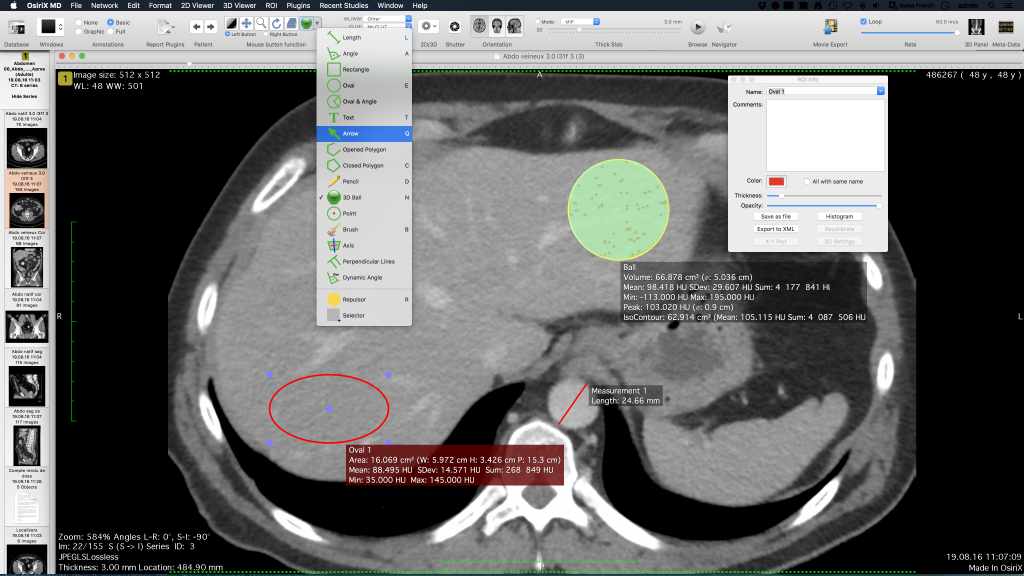
\includegraphics[width=0.9\linewidth]{osirix}
    \caption{OsiriX is one of the most popular image viewers used by the radiologists}
    \label{fig:osirix}
\end{figure}



\section{Discussion about presented workflow}
\subsection{The good parts}
\subsubsection{Viewer software provides expected functionality}
Viewer software has a very stable position on the market and is perfectly tailored to the needs of a radiologist. It often uses advanced techniques of computer graphics to present patient's body as accurately as possible.
\subsubsection{PACS systems provide centralized place for storing images}
They implement functionalities that allow for archiving medical imagery. Lifetime of medical images is controlled by the government and these systems must take this into account. PACS also make it easy to distribute images not only withing local networks but also to any doctor who has the remote access granted.  
\subsubsection{RIS systems make it easy to exchange data between physicians}
There is no need need for the radiologist to deliver the radiological report to the other physician personally as it is done automatically. Also, RIS systems provide good means of presenting medical records from different medical specializations allowing for interdisciplinary diagnostics. 
\subsection{The bad parts}
\subsubsection{Focus on text rather than semantics}
It is expected that the radiologist will produce a consistent, ordered report by means of text editors. Some RIS systems provide basic text formatting functionality like italicization, underlining but they are limited to the textual presentation of the report. There are no means to encode relations in this representation.
\subsubsection{Each radiologist has their own style of writing}
Usually there are no structural expectations about the resulting report. Each radiologist can have their own style of writing, order of organs observation, text formatting. This leads to the waste of time as people who read the report have to make some effort to infer the meaning from plaintext. 
\subsubsection{Selective description}
It is very frequent that radiologists include in the report only things that they consider bad for the patient. This makes the report more goal-oriented but it means that it is useless to get to know the overall state of patient body.
\subsubsection{Copy-paste}
Radiologists try to solve the problem of typing on their own by crating templates that contain certain pathologies listed and what they do is execution of the commonly called 'copy-paste' method to create report content. Sometimes they do not notice parts of copied text that are different from the actual state of the body, so the reports may contain observations that are false. 

\section{Other ways to create radiological reports}
In many English-speaking countries the workflow of a radiologist differs in the way the radiological report is generated. A radiologist may record their voice while describing the imagery vocally. The recordings are then transcribed using either speech recognition algorithms or manually by technologists. Having a good skill of typing by a radiologist is not required, only knowledge to interpret imagery is used. This approach, however, has some architectural disadvantages. More personnel is needed -- technologists, who transcribe the recorded voice\cite{speech-impact}. Also, it is difficult to make changes to what has been said. In some cases, a mistake can made while transcribing the text \cite{speech-africa}.

\section{Problem definition}

After analyzing bad parts of the presented workflow and general situation on the market -- demand for radiological services increases but the number of radiologists appears to be constant, the author decided to design and implement a system that would be used by radiologists to encode semantics of diagnostic imagery in a form that can be easily transformed to the human readable form, analyzed by algorithms. 





\chapter{Description of the proposed solution}
\section{General idea}
\subsection{Area of interest}
The system that is proposed in this thesis focuses entirely on the part of the typical radiological workflow in which a radiologist focuses on the textual description of what can be seen in the diagnostic imagery.
\subsection{Contextual suggestions}
The author analyzed several hundreds of anonymized radiological reports and observed that a lot of time could be saved, if a radiologist would at any time select text fragments from a predefined set of possibilities that are appropriate to the current context. This approach can be seen in the way Integrated Development Environment (IDE) for statically typed languages (e.g. Visual Studio supporting C\#) are suggesting what the programmer can write based on the namespace, class, scope they currently edit.

In the case of programming language the problem is defined in a more strict way. They are very often supported by definitions of formal grammars \cite{csharp-spec}. Radiological reports, however, are written using  natural language, so there always exist some exceptions.


\section{Assumptions}
After observation of actions taken by radiologists while working in environments like hospital, medium-sized clinic, independent teleradiological practice the following assumptions are suggested:
\begin{itemize}
	\item Radiologists prefer using mouse to keyboard
	\item The user interface of the program should be simple 
	\item Reports must be rendered in a way that allows for copying using clipboard as radiologists developed custom ways to save drafts of reports.
	\item The system should allow for exporting reports into formatted text and pdf
	\item Text formatting should be based on semantics that is encoded by a radiologist.
	\item The system should favor reports that describe the whole state of body, not only organs in bad condition.
	\item The system should allow to automatically include in the report segments of text that are (almost) always used (sometimes due to some legal regulations).
	
\end{itemize}
\section{Goals}
\begin{itemize}
	\item Minimize the time radiologist uses keyboard
	\item Split report into structural parts that allow to express description of patient's state.
	\item Any fragment of templated text should be editable. 
	\item Maximize number of reports that can be generated by a radiologist in a unit of time.
	\item At any time allow to include
\end{itemize}


\section{Proposed reporting ontology based on ideas from DICOM SR and HL7 CDA}
In order to provide context for the radiologist at any given moment, it is proposed to split report into the following nested structures:
\begin{enumerate}
    \item Examinations -- single report may have many of them
    \item Organs -- single examination may have many of them
    \item Properties -- single organ may have many of them
\end{enumerate}
Figure \ref{fig:report-semantic} shows how report structures relate by semantic relations.
\begin{figure}
    \centering
    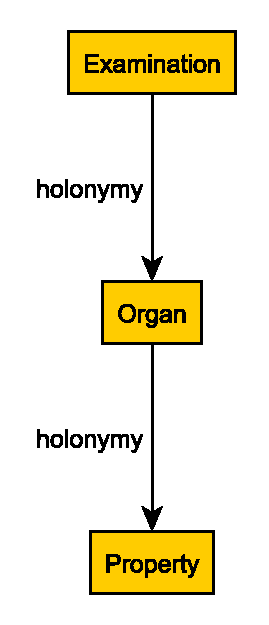
\includegraphics{report-semantic.pdf}
    \caption{Structure of a radiological report created \label{fig:report-semantic}}
\end{figure}

\begin{figure}
    \centering
    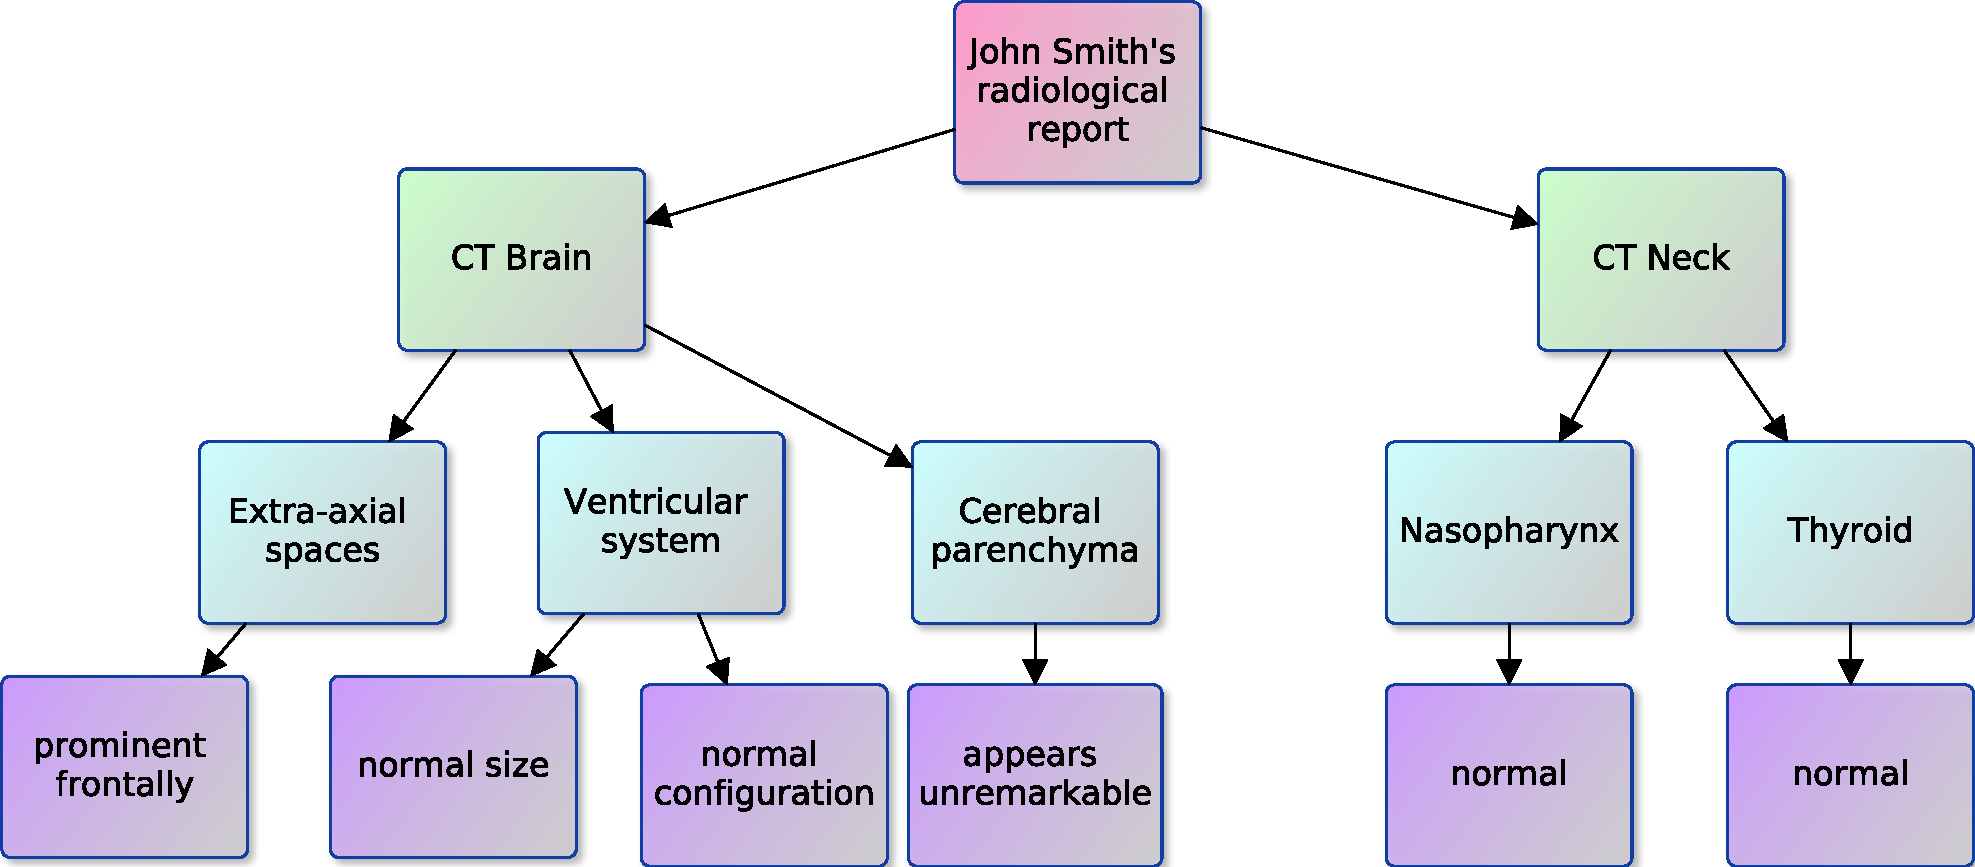
\includegraphics[width=\linewidth]{report-tree.pdf}
    \caption{Structure of a radiological report created \label{fig:report-tree} using proposed system. For simplicity, only names of nodes are presented (associated metadata were omitted)}
\end{figure}

By using this ontology, a radiologist can create a report that is similar in structure to a tree (as it is presented in figure \ref{fig:report-tree}). At any given moment, the doctor modifies the tree at a single level, which allows for suggesting what are the items that can be included. The idea was taken from statically typed languages which, thanks to their strictness, allow for coding with smaller number of mistakes at the lexical level \cite{static-lang}.

\section{Workflow of a radiologist who uses the proposed system}
In figure \ref{fig:report-workflow} a typical workflow of a radiologist is represented in the form of a flowchart. 
\begin{figure}
	\centering
	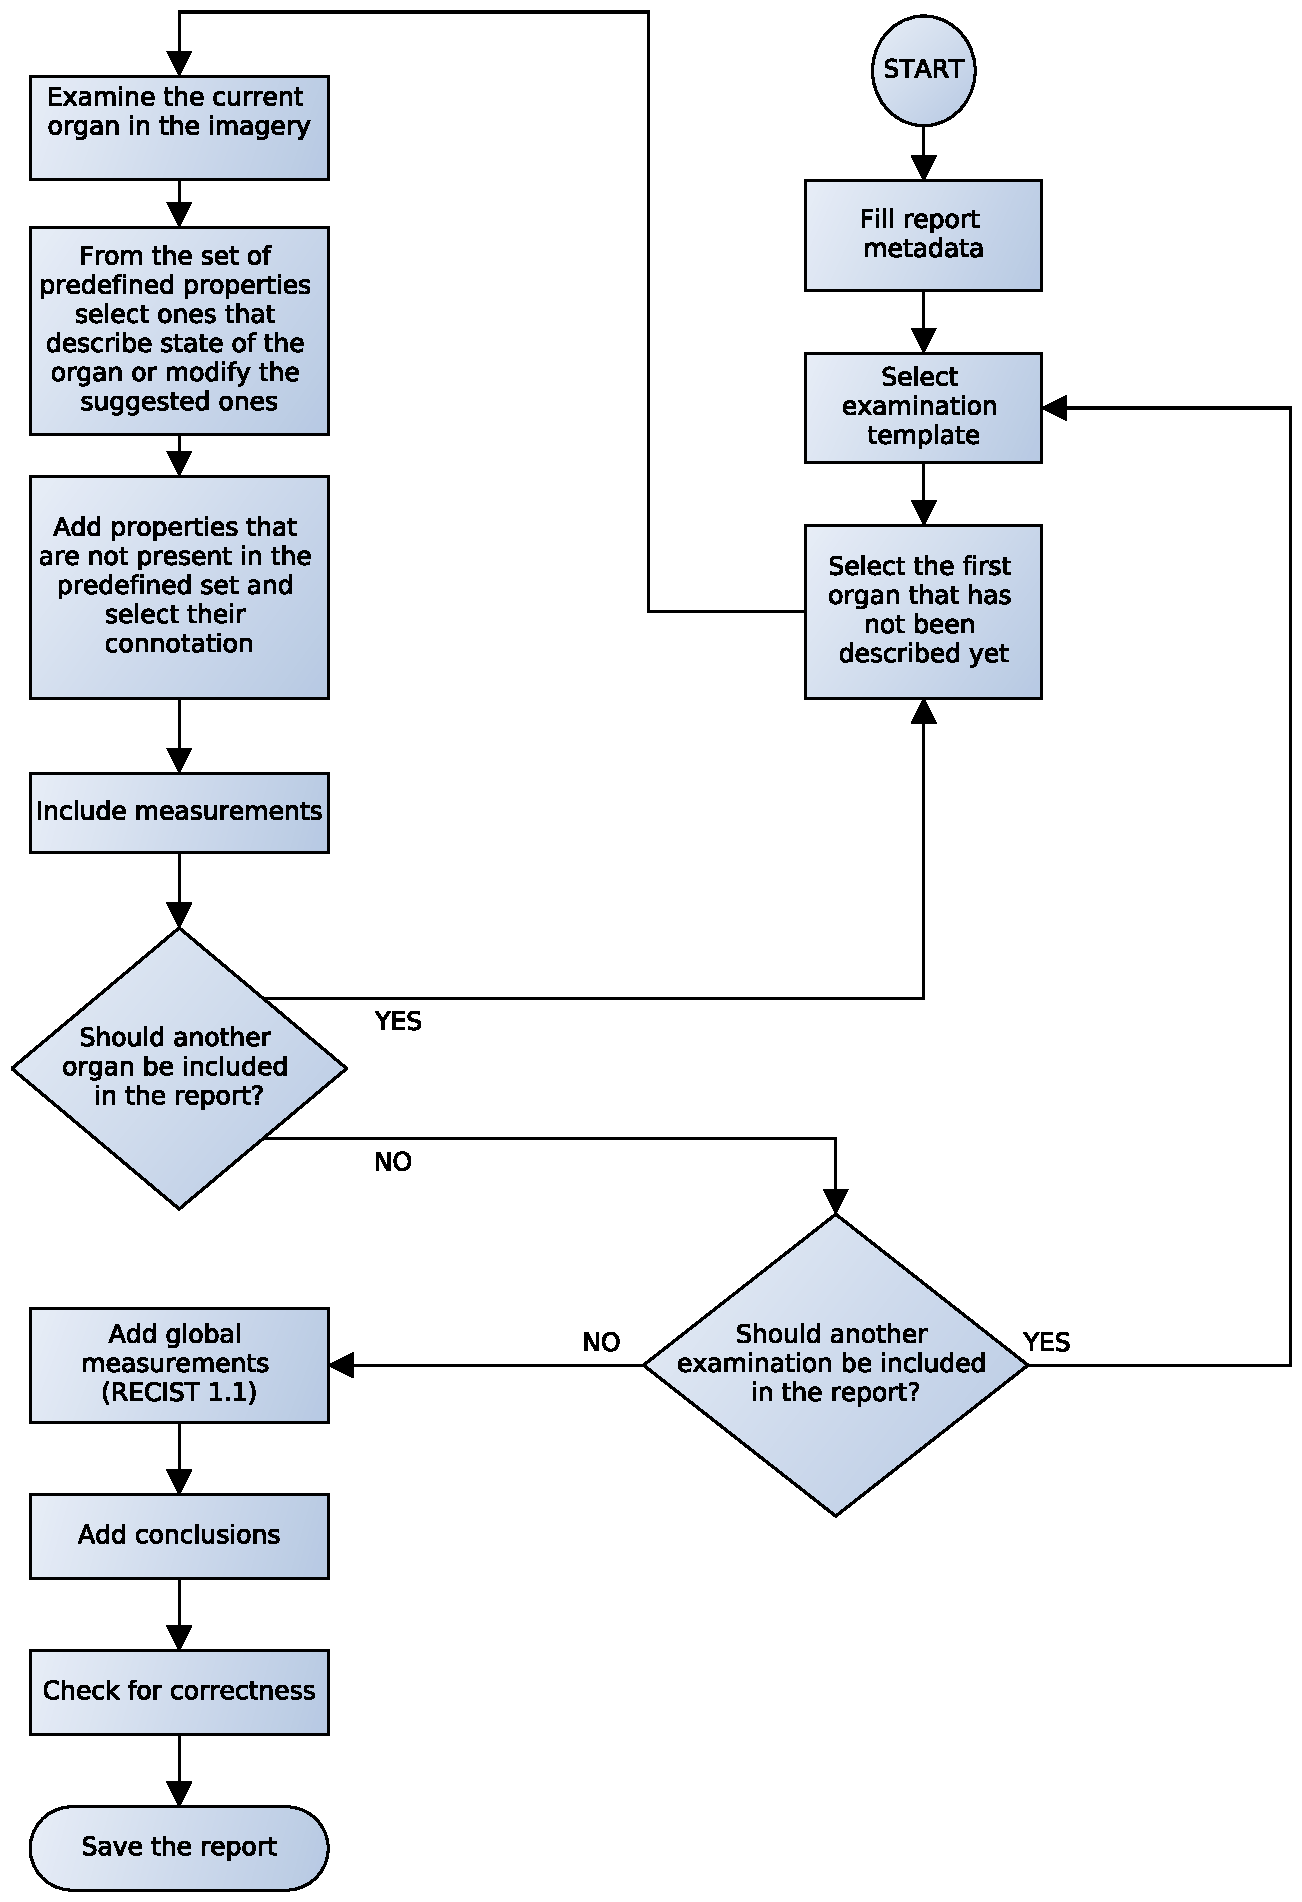
\includegraphics[width=\linewidth]{report-workflow.pdf}
	\caption{Workflow of a radiologist who uses the proposed system to create contents of a radiological report.
		\label{fig:report-workflow}
	}
\end{figure}


\subsection{Connotation}
Moreover, each property has a semantical attribute called connotation. Connotation is used to highlight the impact of this property on the result of the organ and examination. This attribute can have one of three values: positive, negative and neutral. 
\subsection{Metadata}
Report may also contain some metadata which can be used identify the patient whose body is described in it. Shape of these pieces of information strongly depends on the RIS system used in a clinic. These pieces of information have no special influence on the semantics of report so it has no detailed description in this work.

Names for these ontological structures were chosen so it is easier for radiologists to imagine what they describe, however, they can be used not strictly (e.g. in CT scan as an organ one may include details about intracranial hemorrhage which is a kind of bleeding within the skull \cite{ich} but not an organ in its very meaning)

\section{Examination template}
Examination template (or simply 'template') consists of an ordered list of all organs that could be described with all and some portion of metadata used for filtering like category, discipline. Each organ in a template has an ordered list of all properties that can describe it. Every property can have connotation predefined. 

\begin{figure}
    \centering
    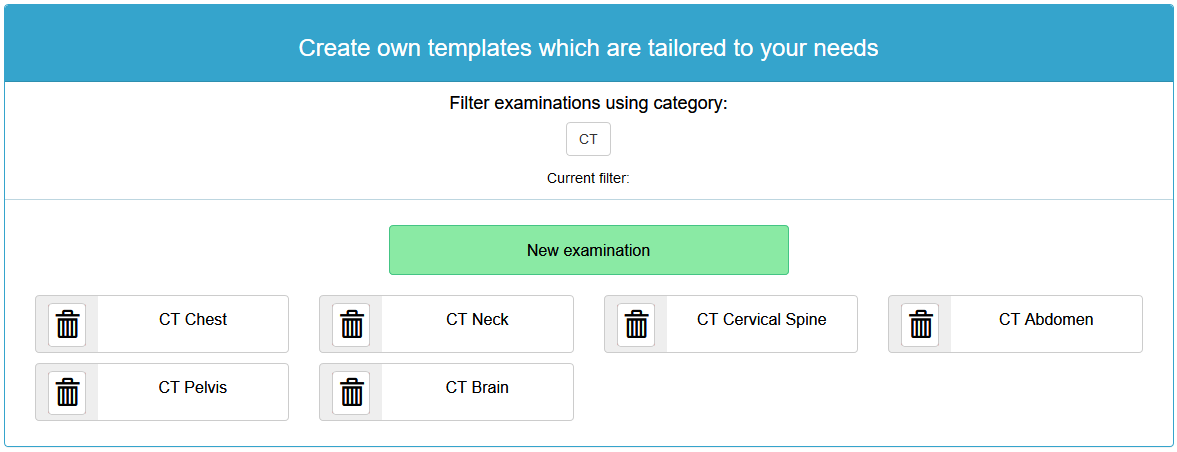
\includegraphics[width=0.9\linewidth]{templates-list}
    \caption{List of templates that can be edited by the user\label{fig:templates-list}}
\end{figure}
\begin{figure}
    \centering
    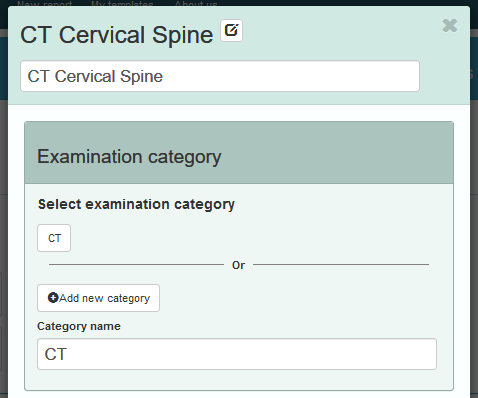
\includegraphics{template-metadata}
    \caption{GUI used to edit template metadata \label{fig:template-metadata}}
\end{figure}
\begin{figure}
    \centering
    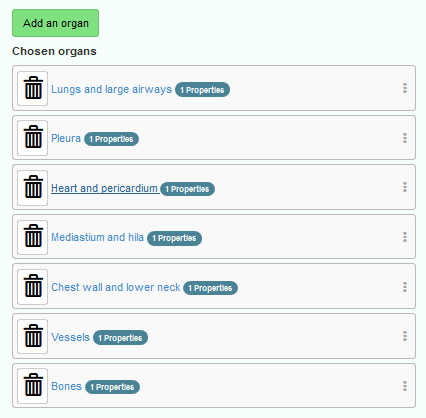
\includegraphics{template-organs-list}
    \caption{GUI used to edit organs \label{fig:template-organs-list}}
\end{figure}
\begin{figure}
    \centering
    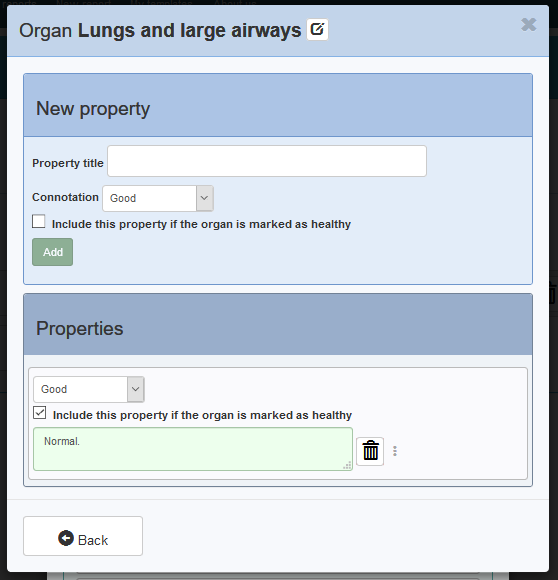
\includegraphics{template-property-list}
    \caption{GUI used to edit properties of an organ. User can predefine connotation and tell the program that this property can be automatically included if the organ is marked as healthy \label{fig:template-property-list}}
\end{figure}

Examination templates can be prepared by the leader of radiologists team, so the team can use common language to describe diagnostic imagery. Templates prepared by the leader constitute the so called set of public examinations.

If a given template is not sufficient for a particular radiologist, they can  create their own template from scratch or extend the existing one (an action that for some people can resemble forking a repo in git \cite{forking})




\section{Productivity improvements}
\subsection{Using templates}
The goal to increase productivity of a radiologist is achieved mostly by decreasing the average time a doctor types on keyboard. By the usage of examination templates, the time spent to create the schema of the report is shifted from the doctor to the leader of the radiologists team. It can take a lot of time to create a template that is both universal and correct but it is a one-time-only investment. The more templates are created using a template, the more it pays off in the long run.

\subsection{Mark organ as healthy}
In the proposed system, each property has additional attribute (it can be set in template editor) named "include if organ healthy". When a radiologist creates a report, an organ can be marked as healthy, which means that all properties that have this attribute set to true are automatically included in the report. This allows to quickly add properties that are very commonly used. 
In order to minimize the possibility of inclusion a  property that does not correspond to the actual state of patient's body, only properties with positive connotation can have this attribute set. 

\subsection{Calculators}
There exist many standardized numerical methods used to asses whether values of certain parameters are in the range suggesting poor health condition, e.g. one of the most popular parameter is the body-mass-index (BMI) which is calculated using formula:
\begin{equation}
BMI=\frac{mass}{height^2}
\end{equation} 
After calculating this index, a radiologist has to look through tables to check whether the value is usually attached to people with obesity or not. 
BMI is one example of hundreds techniques used by doctors. It is not integrated, however, within the proposed system.

\subsubsection{RECIST 1.1}
During the design of the proposed systems several radiologists who specialize in oncological medicine reporting suggested that a method called  Response Evaluation Criteria In Solid Tumors (RECIST 1.1) is of special importance to them. This method is used to assess whether tumors in cancer patients improve, stay the same, or worsen during treatment \cite{wiki-recist}. As there are hundreds of similar methods used by radiologists, it would be impossible to implement them in the proposed system all at once, so it was decided to use RECIST 1.1 as a proof of the concept of calculators that can be used in structured reports.
A radiologist, while creating a report, can measure size of lesions and write down the results of measurement in the report. Proposed program should recognize that the numerical value represents a measurement and should suggest whether it should be included in the calculation of RECIST 1.1 or not.

\section{Reporting quality improvements}
\subsection{Standardized nomenclature}
There exist several attempts to standardize the language doctors use to describe precisely medical imagery. Templates created for the proposed structured reporting system can be created with the help of terminologists who specialize in systematized nomenclatures like SNOMED and LOINC to create reports what can lead to improved reporting quality as a radiologist does not have to explore huge volumes of precise textual definitions of terms used. 
\subsection{No repetitions}
Templates can be interpreted as TODO-lists containing tasks which have to be done while describing medical imagery, so a radiologist can be sure that nothing was omitted or no item appears twice in the report as a result of a mistake.
\subsection{Reports have ordered list of elements}
Reports created using the proposed system can be represented as trees, nested lists of items, so it is easy to spot relationships between properties and organs and also differences between two reports describing one patient.
\subsection{Highlighting the most important pieces of information}
The most important pieces of information can be highlighted using proper value of connotation. When one of properties of an organ should be interpreted as a main cause of health problems it is marked as a pathology. When the report is then rendered as a document, this property can have e.g. different font color, some text-decoration element or different background color.
\subsection{Shift from difference reporting to the current state reporting}
There exists practices quite popular among radiologists mostly from smaller clinics that are considered as bad among professionals. One is to include in the radiological report only properties of body which they consider as bad for patient's health. Due to the subjective nature of the report there were cases when a radiologist skipped a finding that was important stating the patient was healthy leading to more difficult and expensive treatment later.
There were also cases when a radiologist was unable to compare current state with descriptions of several images that were taken at different times, only with the last one. The doctor stated that there is a progress in treatment, but in comparison to the second from the last description, the health condition worsened. \cite{risk-management}
Templates created using the proposed system can favor radiological reports that are more self-contained -- they describe both bad and good properties of patient's state.

\subsection{Compare reports}
Having a previous report, a radiologist can create another one that will be an update to the former. This procedure is often applied during chemotherapy to see whether tumors react to the treatment. A software functionality that allows the radiologist to introduce small changes to the report without rewriting it, would increase the quality of reporting as the resulting report would be still self-contained.

\section{Integration with existing systems}
As there are many ways to store radiological reports. Many radiologists work remotely for several companies that have different RIS systems. It is very difficult to integrate the system with all of the systems as it requires cooperation of both developer of the proposed system and the developers of the RIS system. 

The approach taken by the author is very robust, works for all of the systems used nowadays but is not very elegant from the point of view of software engineering. 
After generating the report using the proposed system, it is the radiologist's duty to manually copy the resulting report to the RIS system. It is simplified in a way that the report is automatically copied to the clipboard after clicking on its content.

On the other hand, the proposed system was designed in a way that makes it easy to create communication channels that can be used to integrate this system with existing RIS systems. 









\chapter{Implementation}
The proposed system was implemented as a web application. It is split into two parts: frontend and backend. Frontend  
\section{Technological stack}

\subsection{Backend}
\subsubsection{C\#}
As a main technology that is used to structurize data that is displayed to the user or received from them, ASP.NET C\# framework was used.
C\# is an imperative, strongly-typed, object-oriented language that is used on the market to create enterprise software. There exists a lot of high quality tooling that makes development in this language faster and less error-prone.

\subsubsection{ASP.NET}
The ASP.net application is created using MVC pattern (Model-View-Controller) that is widely known for helping to create applications that consists of loosely coupled, pluggable components. Some interactions with user interface result in HTTP requests that are then mapped by the server to routes that are forwarded to Controllers. Controllers are used to react to user action, instantiate proper classes which implement application logic (they are part of the Model), feed them with sanitized and validated user input and invoke proper methods. When the results of execution are present, Controller finds a View that is expected to be used to present results to the user. View can be treated as a template for the data that is returned from Controller. It can be an ordinary HTML file with placeholders for certain pieces of information (it can also include formatting) or even JSON or XML documents that are only concerned with shape of the data, not the formatting.

\subsubsection{Entity Framework}
Entity Framework is a set of libraries that is used to create high-level abstract model using C\# that are then converted to sets of relations and attributes of the underlying DBMS. It can also be used to transform LINQ constructions to SQL queries taking into the account vendor-specific features of many DBMS.
The act of first creating C\# classes that represent Model and then automatically converting it to the database relations and attributes (scaffolding) is called Code First Approach. It can be especially useful when the schema of database changes very often. When changes are introduced to the code representing Model, Entity Framework can be used create a migration  -- set of transformations for DB schema that after applying to the DB will keep code and schema synchronized. 

\subsection{Database}
MSSQl server is used as a DBMS because it is a battle-tested, well-documented solution that can be easily paired with ASP.NET and Entity Framework's code generation methods are best optimized for this particular DBMS. 

\subsection{Frontend}
Not all interactions with the application result in HTTP requests sent to the server, many of them are about shaping data that has already been received from the server. In order to make use of this fact main part of the application -- tabs: New Report and Templates were developed as a Single Page Applications (SPA) in order to minimize the time that user has to wait between actions they take. Technologies used in these parts are JavaScript and AngularJS framework. 

\subsubsection{JavaScript}
It is a very popular scripting language that can be executed in any popular web browser. Version of the language used in this project is ECMAScript 5.1 compliant. 
\subsubsection{AngularJS}
AngularJS is a JavaScript framework that helps with building MVC SPA aplications. It has several mechanisms like two-way-binding that reduce size of the code needed to implement Create, Read, Update, Delete (CRUD) functionality.


\subsubsection{Razor views}
The remaining frontend subpages are generated using view engine present in ASP.NET called Razor. These views are responsible for interactions like logging in , registration (backed with ASP.NET identity mechanism), listing reports, searching for particular report etc. They are generated on the server side and sent to the user as HTML and rendered by the browser.
 


\section{Internationalization and localization}
The application was designed to be accessible by radiologists from many countries, so support for many languages is one of its core functionalities. The application automatically detects user preferred language by looking into user browser settings. Each of the most popular Internet browsers allows users to specify list of preferred languages used by webpages. The presented solution scans this list and chooses first language it supports, if there are no languages in the list that are supported, English language is presented to the user by default. Figure \ref{fig:language-preferences} shows how this list can be manipulated in one of most popular web browsers.
\begin{figure}
    \centering
    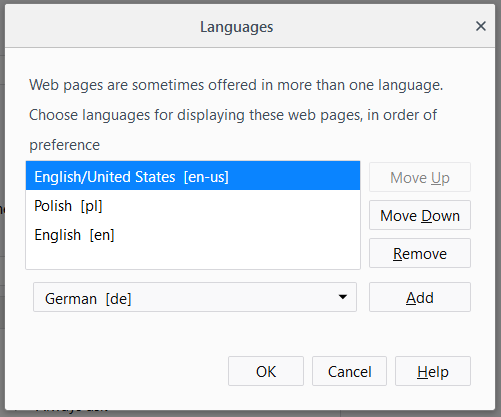
\includegraphics[width=0.6\linewidth]{language-preferences}
    \caption{Language preferences list present in Firefox 54\label{fig:language-preferences}}
\end{figure}

At the back-end there are dictionaries for each supported languages that contain mapping name -> value. 
In Razor views names are used to specify where particular piece of text should be placed. During HTML generation, the application resolves user language and refers to proper resource. Figure \ref{fig:language-dictionary} presents contents of a dictionary for ReportWizard for Polish language. Adding support for another language is simply providing values for existing names in the dictionary.

For SPA parts of the program the situation is slightly different as DOM elements representing most of their content are generated at the user side with the help of AngularJS. In order to have single source of truth about translations, it was decided to serialize contents of dictionaries to JSON format, and send it to the user with page template. At the front-end the translation dictionary entries are deserialized and made available to JavaScript functions. This solution makes it faster to edit and version translations as they are kept in a single place. One of drawbacks can be the performance of this solution, but it was measured that for number of dictionary entries used in this application, the decrease in performance is negligible.
 
\begin{figure}
    \centering
    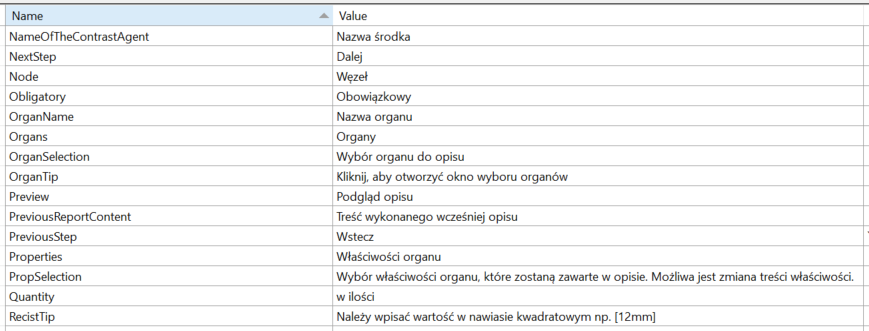
\includegraphics[width=1\linewidth]{language-dictionary}
    \caption{Dictionary for Report creator for Polish language\label{fig:language-dictionary}}
\end{figure}
\section{Templates}
Templates can be manipulated by the user at the examination level. Users can create them, edit, remove. In order to keep things simple and less error-prone, they are treated as immutable in the database. If user edits a template, the previous version of the template is deleted and template version with edits is inserted into database. The only thing that is not changed in this process is its primary key. This makes reasoning about database queries much easier and has satisfactory performance for templates used by most radiologists. Thanks to the use of database transactions, one can be sure that removing contents of an existing template and inserting contents of a template with modifications is performed atomically.

\subsection{Feeding front-end with data from database}\label{templates-immutable}
After browser finishes loading static files (scripts, fonts, etc.), an additional HTTP request is created to download report templates attached to the current account. Server handles the request by querying database, instantiating model classes that correspond to the data received from database. Finally, server serializes reports data to the JSON format and sends it to the front-end. When front-end receives JSON data, a success callback is invoked and sets the data as current view model. 
From now on user can edit any existing template: add properties, organs, remove them, change connotations, reorder elements. Thanks to the two-way-binding mechanism, user interface can be directly connected with references to the fields of an object so the developer can focus on the visual representation of the editor. In order to make editor more robus, lenght of text contained in it is measured on each onChange event and its height is adjusted, so all its contents are visible to the user.
\subsection{New Examination}
User can create new template by clicking on New examination button. Then they are asked to input title of new examination. One of requested features was the ability to copy contents of existing examinations what is similar to forking in git. In order to achieve this, when modal with new examination's title is opened, front-end loads from server list of user-owned examinations concatenated with list of publicly-available examinations. The latter allows users to quickly customize templates prepared by the administrator.

\subsection{Edit examinations}
On page load all templates that are owned by the user are downloaded, so editing template is setting is as a current template of the editor. Any modification can be applied: renaming, reordering of elements, setting connotation, etc. When user clicks Save button, actions related to the immutability of templates described in section \ref{templates-immutable} are performed.


\section{Report creator}

\subsection{Data loaded lazily}
Report creator is the most optimized part of the application. It is the place where user spends most of their time and it has to respond to any action immediately. It is not easy to predict which examinations will be used in a particular report, so all of available examinations must be ready to be loaded. At the page load, only list of available examinations' titles (user owned and public examinations) is loaded from the server. When the user clicks on examination's title, the rest of template's content is loaded via HTTP call and ready to be modified and included in the report.  
\subsection{Caching at the user side}
If a radiologist is specialized in a particular field, they have subset of examinations that they describe most often. Loading them separately each time they create a report would be a waste of time. In order to solve this issue, a caching mechanism at the user side was designed. After loading, JSON data describing examination elements are saved to the storage managed by the browser called localStorage. It is a dictionary-like storage that can be used from JavaScript to save string values. When user tries to open an examination, the localStorage cache is checked whether this examination is present. If the examination is in the cache, it is immediately shown to the user. Otherwise, an HTTP request to the API is issued to download data.
\subsubsection{Cache invalidation}
As templates contain no sensitive information, they can be stored in localStorage without restrictions regarding synchronization of cache invalidation with session expiry time. However, the invalidation has to happen when user updates an examination in the Templates tab. In order to keep things simple, the whole cache gets purged anytime user navigates to this tab. 

\subsection{Editing functionality}
As user moves on in the levels of structure, the program signifies this by opening modals one on top of another. This results in the following behavior: when user makes decisions that have the biggest impact on the shape of the report -- edits report meta-data, selects examinations that will be used -- the program is at the 1 st level of depth, no modals are present.
When user decides to include an examination, a modal is opened hiding all information that is not necessary at the moment and the user is shown list of organs with preview of the report.

Workflow is designed to favor selecting Examinations/Organs/Properties from predefined sets. It was measured that with suggested use of the templates on average 82\% of report's content can be generated from template contents. As most of the content can be added to the report by simply clicking on a check-boxes, a lot of thought went into designing interaction model that allows radiologists to look at sequence of suggested elements and make a binary decision 'yes' or 'no' whether an element should be included in the report or not. 
As the program can be used on any device, it can be interacted using mouse or using touch. When the program is executed on a device with mouse, the font-size and check-boxes are smaller as user uses mouse to precisely click on them. When the program is executed on a smaller device like tablet or smartphone, some elements are shrunk but check-boxes become bigger, so it is easier to tap them. 

\subsection{Predefined but modifiable}
In some situations edits must be made to the predefined pieces of text. This was solved by putting any report text in a slightly customized textarea that is attached to AngularJS context. The textarea is aware of the length of text it contains and automatically fits its height to show the whole text to the user at any time.


\subsection{Live preview}
It is crucial for the user to always be aware of the impact of edits they make to the report contents. Live preview was designed specifically to solve this. Any significant change of context or report contents send an event to the function that filters elements that were selected and generates report's textual representation. As this function has computational complexity $O(n^3)$, it cannot be left to AngularJS to decide when it should be called (infamous \$digest cycle \cite{angular-digest}) as it would have a severe impact on performance. AngularJS internally observes arrays of data that are attached to its scope to look for changes, so it was decided to call this function only in several situations, e.g. when report-context is switched, a property is checked etc. but not on every single text-change of the report. This allows the radiologists to have a close-to-live preview of resulting report while focusing on selecting predefined pieces of text.

\subsection{Storing a report in the database}
This is a very important decision from the architectural perspective. Format of the saved report can impact the performance of retrieving saved report, interoperability with other systems, etc. The format of stored report could be a topic for a very broad discussion. In order to maintain the simplicity of the whole project, it was decided store JSON representing the report in the database. Many of the DMBS have special functionalities that are based on ideas used in NoSQL databases, especially document databases to allow for storing JSON objects, validating and querying them as if they ware part of the relational data. This makes it easy to store data that can have numerous optional fields. Unfortunately, SQL Server does not support storing JSON objects natively (Microsoft calls their limited way of supporting this format as \textit{built-in JSON support}\cite{microsoft-json-support}), however, it is possible to store JSON string representation in a column of NVARCHAR and then
Relation that represents reports' data has a json\_body attribute of type JSON
\section{Report history}
Report history is a part of the program that is used to list saved reports, search for particular ones, request pdf version of reports, sending report content via email. users can invoke on existing reports such important actions as editing them, deleting them, comparing them. As one user may have created thousands of reports using this program, this section paginates reports, so not all of them are listed at a time. There are 10 reports per page and user can increment index of the page they are currently viewing or decrement it. 
One useful feature is grouping reports by title. This is useful when user has the convention of naming that report's title is always name of the patient (most of the current users of the program do it in this way) as they can see and count reports for any user organized in groups. 

\section{Compare reports}
This feature strongly depends on the mechanisms included in the Report creator. It copies metadata of an existing report and creates a new report using it. Content of the old report is presented to the radiologist as a reference and it is also copied as a basis of a new report. When the doctor makes some changes to the contents of the report, only the new version is modified. This allows for fast creation of a report that has only small portion of fragments modified when compared to the previous one.

\section{Deployment strategy}

Figure \ref{fig:continuous-deployment} presents the sequence of actions and set of subjects that are required to deploy the application.
\begin{figure}
	\centering
	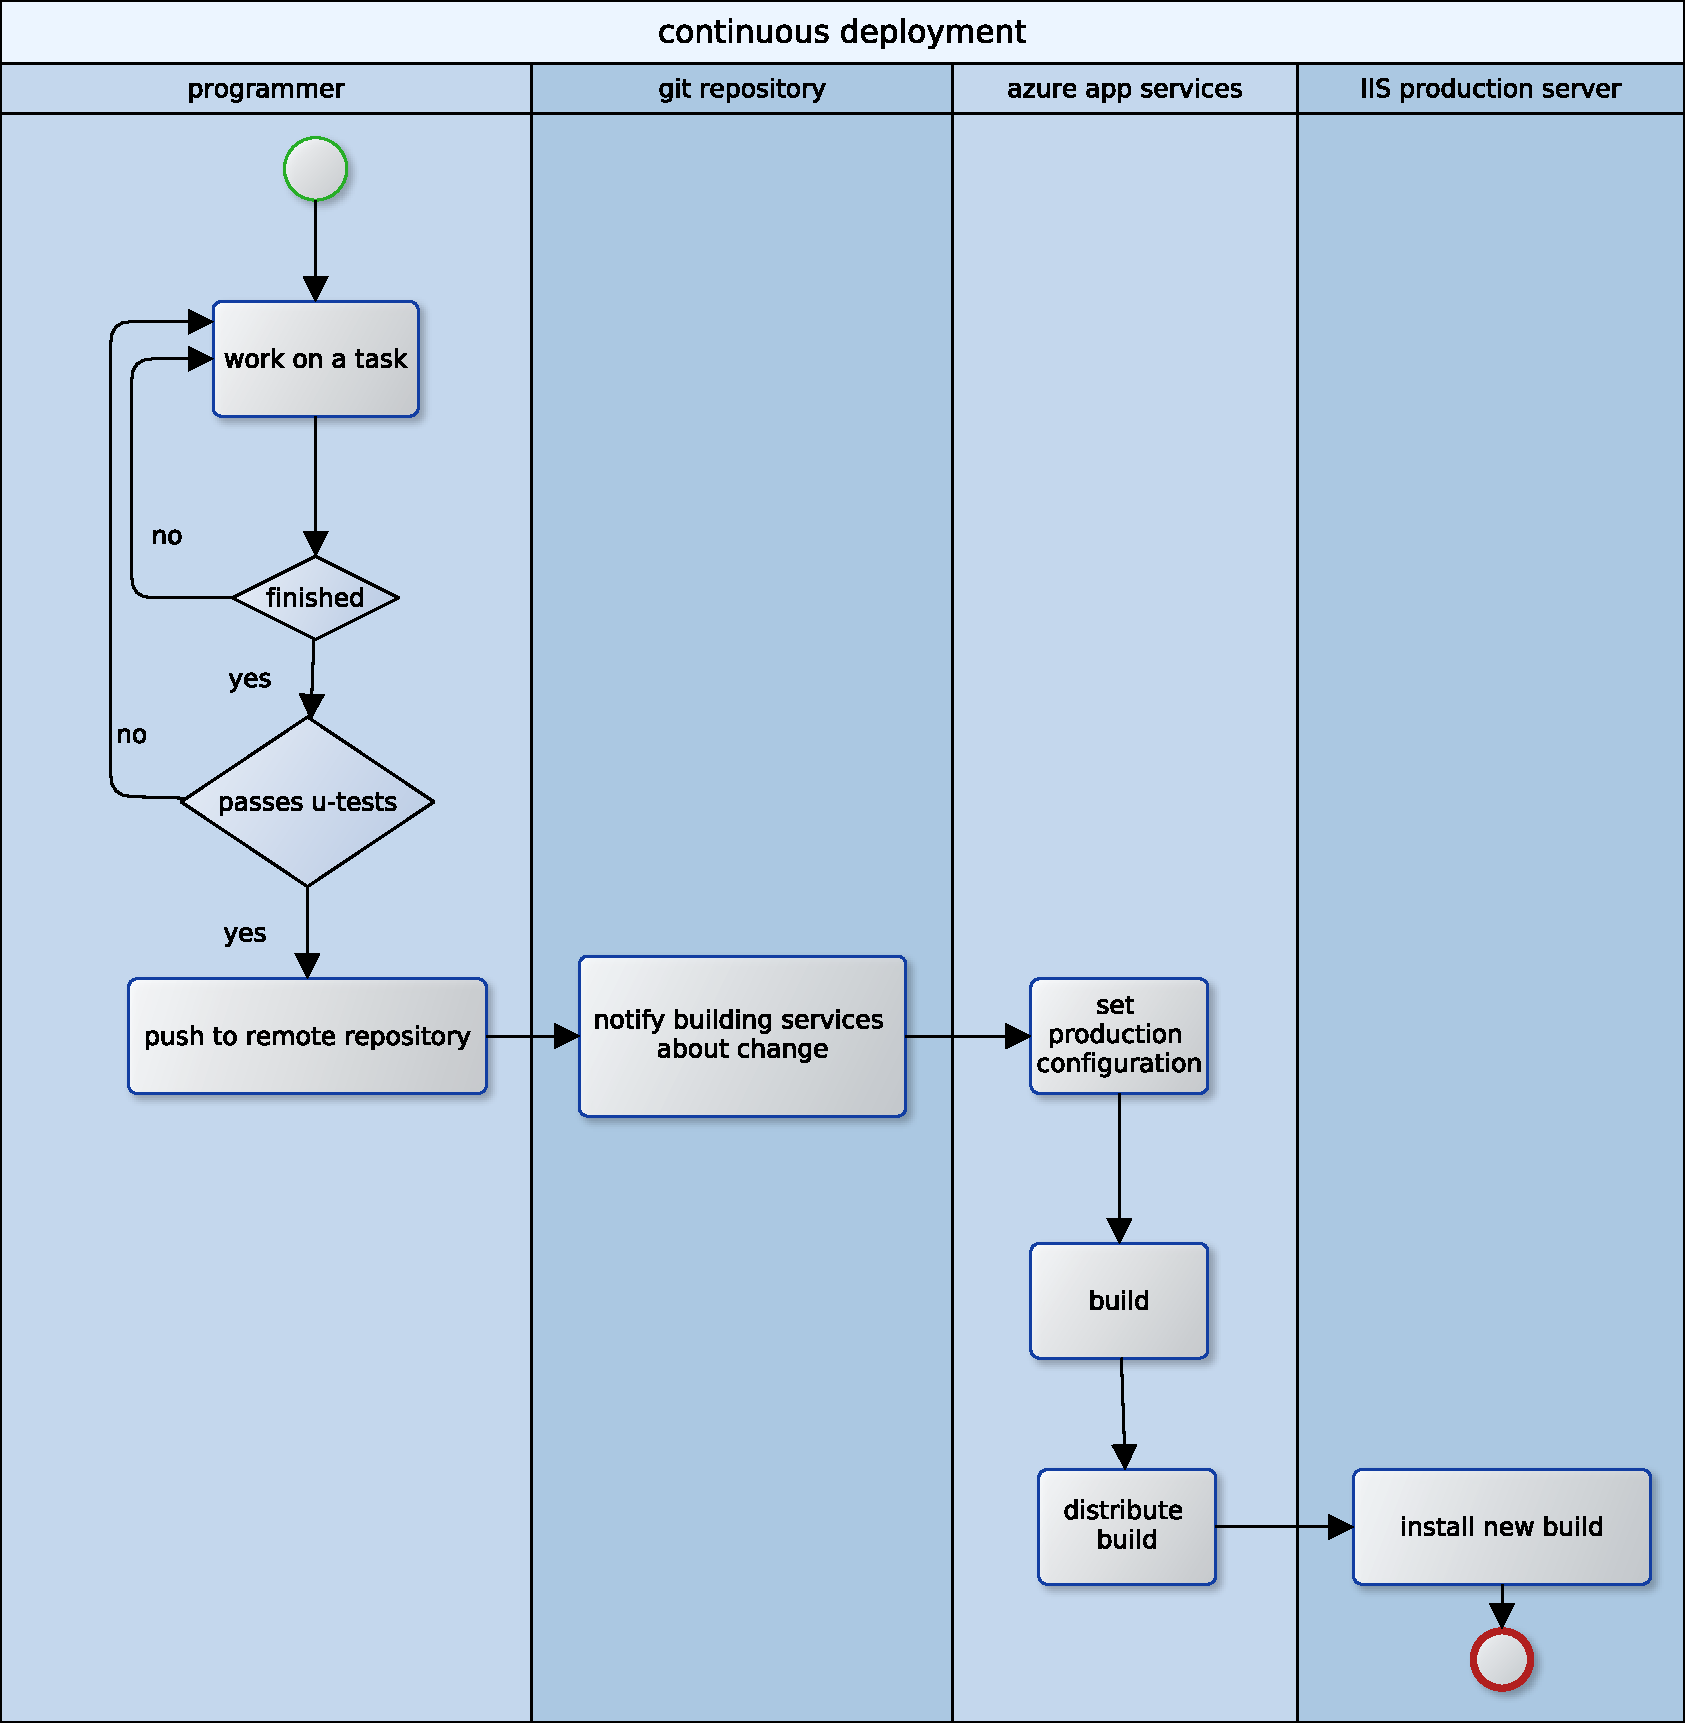
\includegraphics[width=\linewidth]{continuous-deployment}
	\caption{Continuous deployment setup makes it faster to distribute new builds to the production servers.
		\label{fig:continuous-deployment}
	}
\end{figure}

\chapter{Testing and verification}



\chapter{Validation of the proposed solution and examples of places where it was used}
\section{Teleradiologists}
Structured reporting system is being used by several independent teleradiologists in Poland as their main text editing tool. They receive reporting requests with images they are asked to describe. They use several RIS systems from different vendors to store reports they generate. Most of them simply copy and paste reports from the System to the RIS systems they use.

\section{Hospital}
Proposed system was used in hospital in Wieliszew by a group of radiologists who specialize in oncological reporting. They provided me with precious feedback and many of their suggestions were included in the system. 
The following paragraph is an opinion about the proposed system authored by Ms. Maria Uliasz, MD–PhD, Director of Radiology at Dziekanów Leśny hospital:
\blockquote{
Health informatics supports almost every activity carried out when examining state of patient’s body as techniques used in modern medicine generate a lot of data that must be presented to a proper person at proper time.
On the other hand, medical diagnostics forms a basis for all medical specializations and has been rapidly advancing for more than 100 years thanks to the interdisciplinary cooperation between professionals. Numerous breakthroughs in the fields of computer imaging and medical diagnostics dated back to the end of 20th and the beginning of 21st century allowed for dynamic development of such imaging techniques as: computed tomography scan, magnetic resonance imaging, positron-emission tomography and nuclear medicine. 
Speed and diagnostic accuracy are crucial factors in the process of diagnosing patients. The process consists of actions like capturing data from patient’s body, creating radiological report and delivering it to the recipient – physician.
Reporting system presented by Paweł Paczuski was designed to improve productivity and quality of reports created by radiologists. The program simplified significantly typical workflow of radiologists and, by the use of customizable templates, allowed to save a lot of time. This piece of software is especially useful for creating reports for examinations that require a lot of attention from a radiologist, such as: ultrasonography, magnetic resonance imaging, computed tomography scan. 
The user interface of the program is intuitive and guides user through set of activities required to create a report of a very good quality. Thanks to context-aware phrase suggestions, most of the text can be generated semi-automatically but still allowing for modifications at any time while creating a report. Another useful functionality is RECIST 1.1 calculator that automatically extracts measurement from the report’s text and allows for fast and objective assessment of patient’s reaction to the ongoing oncological therapy. The ability to compare reports makes doctors more productive while creating reports that should present how patient’s state changed between two points in time. This greatly shortened report turnaround time for cancer patients who require numerous control exams reports. In the future, I hope for having access to more software tooling that helps doctors, especially radiologists and teleradiologists, be more productive.
The Structured Reporting System could be used as a supplement for Viewer software as a text-generation tool to create coherent, easy to read, well-formatted and typo-free text. Template based approach could be applied not only to diagnostic imaging, but I can see the existence of market for this piece of software in paramedical, educational and juridical applications.}


\section{Large network of clinics}
Structured reporting system is used by a large network of private clinics in Łódź. Integration with their RIS system is being developed, so the systems will cooperate with existing systems to optimize workflow of radiologists.


\chapter{Conclusion and ideas for future}
Ideas implemented in this structured reporting system are very simple from the theoretical point of view. In fact, template-based text generation existed for years and can be found in most of the programs developed by humans. However, even such simple methods, supported with well-thought user experience design can give satisfying results. 
In the future one could think about a way to generalize the reporting ontology or implement a mechanism to create custom ontologies to provide tools that would allow to encode a hierarchy of an arbitrary depth. After obtaining a well-formed tree representing relations between causes and effects, one could experiment with applying recurrent neural networks (RNNs) to automatically generate report's text from structured data source \cite{recurrent-neural-networks}. Another direction for improvement would be a natural language processing mechanism that would learn typical co-occurrences of report items and would ask the radiologist whether an unusual report content is caused by a mistake made while creating the report or a truly unusual pathology. 

As the program was developed during my first year of studies at Warsaw University of Technology, I had a lot of time to think about pros and cons of the ideas presented in this solution. Some of the improvements were implemented in a commercial product based on some ideas presented in this thesis available at upmedic.pl



%-----------Koniec części zasadniczej-----------

\begin{thebibliography}{11}
\bibitem{bls} https://www.bls.gov/ooh/healthcare/physicians-and-surgeons.htm, accessed 08.10.2017 13:30
\bibitem{ai} M. Recht, N. Bryan, Artificial Intelligence: Threat or Boon to Radiologists?

N1  - doi: 10.1016/j.jacr.2017.07.007
\bibitem{snomed} T. Benson, Principles of health interoperability HL7 and SNOMED.
\bibitem{sr} D. A. Clunie, DICOM Structured Reporting
\bibitem{hl7cda} http://www.hl7.org/Special/committees/structure/index.cfm 
\bibitem{techonologist} https://www.asrt.org/main/careers/careers-in-radiologic-technology/who-are-radiologic-technologists
\bibitem{workflow} https://radiologystories.com/2013/10/31/the-typical-radiologist-work-day/
\bibitem{viewer}
http://www.osirix-viewer.com/osirix/overview/
\bibitem{speech-impact}
S. Langer, Impact of Speech Recognition on Radiologist Productivity
\bibitem{speech-africa} J. du Toit, R. Hattingh and R. Pitcher, The accuracy of radiology speech recognition
reports in a multilingual South African teaching hospital.
\bibitem{csharp-spec}
https://docs.microsoft.com/en-us/dotnet/csharp/language-reference/language-specification/lexical-structure
\bibitem{ich} http://emedicine.medscape.com/article/1163977-overview
\bibitem{static-lang}
    S. Hanenberg, S. Kleinschmager, R. Robbes, É. Tanter, A. Stefik, An empirical study on the impact of static typing on software maintainability
\bibitem {forking} https://help.github.com/articles/fork-a-repo/
\bibitem{wiki-recist} 
https://en.wikipedia.org/wiki/Response\_Evaluation\_Criteria\_in\_Solid\_Tumors
\bibitem{risk-management} https://www.ncbi.nlm.nih.gov/pubmed/3497558
\bibitem{angular-digest} https://www.sitepoint.com/understanding-angulars-apply-digest/
\bibitem{microsoft-json-suppoert} https://blogs.msdn.microsoft.com/jocapc/2015/05/16/json-support-in-sql-server-2016/
\bibitem{recurrent-neural-networks}
http://www2.fiit.stuba.sk/~kvasnicka/NeuralNetworks/6.prednaska/Kvasnicka\_RNN\_exten\_transp.pdf
\end{thebibliography}
\clearpage
\begin{otherlanguage}{polish}
\pagestyle{empty}
\noindent Warszawa, dnia ...............
\vspace{5cm}
\begin{center}
\LARGE{Oświadczenie}
\end{center}
Oświadczam, że pracę inżynierską pod tytułem: ,,Tytuł pracy'', której promotorem jest ––, wykonałem/am samodzielnie, co poświadczam własnoręcznym podpisem.
\vspace{2cm}
\begin{flushright}
...........................................
\end{flushright}
\end{otherlanguage}
\end{document}